% Created by tikzDevice version 0.10.1 on 2017-10-30 17:28:42
% !TEX encoding = UTF-8 Unicode
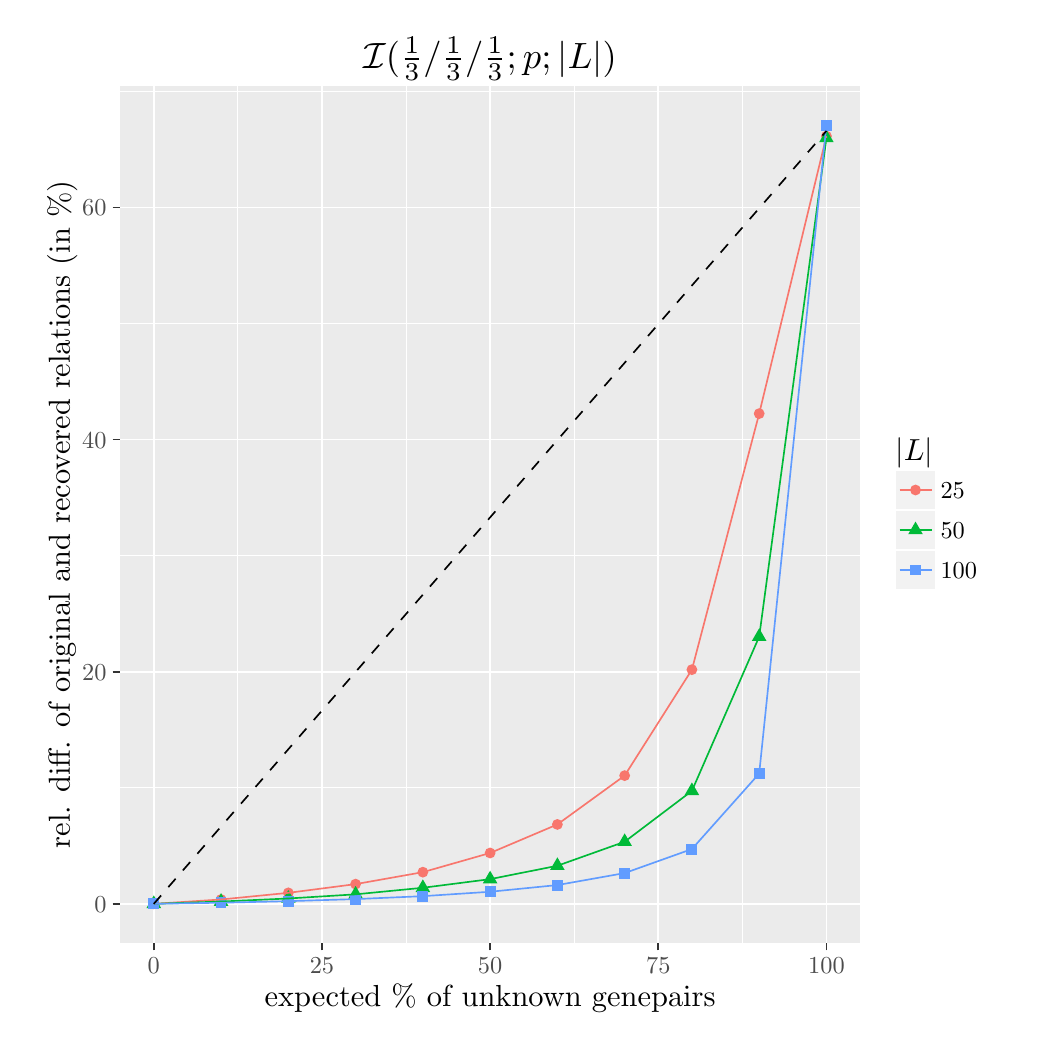
\begin{tikzpicture}[x=1pt,y=1pt]
\definecolor{fillColor}{RGB}{255,255,255}
\path[use as bounding box,fill=fillColor,fill opacity=0.00] (0,0) rectangle (361.35,361.35);
\begin{scope}
\path[clip] (  0.00,  0.00) rectangle (361.35,361.35);
\definecolor{drawColor}{RGB}{255,255,255}
\definecolor{fillColor}{RGB}{255,255,255}

\path[draw=drawColor,line width= 0.6pt,line join=round,line cap=round,fill=fillColor] (  0.00,  0.00) rectangle (361.35,361.35);
\end{scope}
\begin{scope}
\path[clip] ( 33.42, 30.69) rectangle (300.78,340.16);
\definecolor{fillColor}{gray}{0.92}

\path[fill=fillColor] ( 33.42, 30.69) rectangle (300.78,340.16);
\definecolor{drawColor}{RGB}{255,255,255}

\path[draw=drawColor,line width= 0.3pt,line join=round] ( 33.42, 86.69) --
	(300.78, 86.69);

\path[draw=drawColor,line width= 0.3pt,line join=round] ( 33.42,170.55) --
	(300.78,170.55);

\path[draw=drawColor,line width= 0.3pt,line join=round] ( 33.42,254.42) --
	(300.78,254.42);

\path[draw=drawColor,line width= 0.3pt,line join=round] ( 33.42,338.28) --
	(300.78,338.28);

\path[draw=drawColor,line width= 0.3pt,line join=round] ( 75.96, 30.69) --
	( 75.96,340.16);

\path[draw=drawColor,line width= 0.3pt,line join=round] (136.72, 30.69) --
	(136.72,340.16);

\path[draw=drawColor,line width= 0.3pt,line join=round] (197.49, 30.69) --
	(197.49,340.16);

\path[draw=drawColor,line width= 0.3pt,line join=round] (258.25, 30.69) --
	(258.25,340.16);

\path[draw=drawColor,line width= 0.6pt,line join=round] ( 33.42, 44.75) --
	(300.78, 44.75);

\path[draw=drawColor,line width= 0.6pt,line join=round] ( 33.42,128.62) --
	(300.78,128.62);

\path[draw=drawColor,line width= 0.6pt,line join=round] ( 33.42,212.48) --
	(300.78,212.48);

\path[draw=drawColor,line width= 0.6pt,line join=round] ( 33.42,296.35) --
	(300.78,296.35);

\path[draw=drawColor,line width= 0.6pt,line join=round] ( 45.58, 30.69) --
	( 45.58,340.16);

\path[draw=drawColor,line width= 0.6pt,line join=round] (106.34, 30.69) --
	(106.34,340.16);

\path[draw=drawColor,line width= 0.6pt,line join=round] (167.10, 30.69) --
	(167.10,340.16);

\path[draw=drawColor,line width= 0.6pt,line join=round] (227.87, 30.69) --
	(227.87,340.16);

\path[draw=drawColor,line width= 0.6pt,line join=round] (288.63, 30.69) --
	(288.63,340.16);
\definecolor{fillColor}{RGB}{248,118,109}

\path[fill=fillColor] ( 45.58, 44.75) circle (  1.96);

\path[fill=fillColor] ( 69.88, 46.32) circle (  1.96);

\path[fill=fillColor] ( 94.19, 48.72) circle (  1.96);

\path[fill=fillColor] (118.49, 51.87) circle (  1.96);

\path[fill=fillColor] (142.80, 56.19) circle (  1.96);

\path[fill=fillColor] (167.10, 63.12) circle (  1.96);

\path[fill=fillColor] (191.41, 73.44) circle (  1.96);

\path[fill=fillColor] (215.72, 91.08) circle (  1.96);

\path[fill=fillColor] (240.02,129.37) circle (  1.96);

\path[fill=fillColor] (264.33,221.89) circle (  1.96);

\path[fill=fillColor] (288.63,322.16) circle (  1.96);
\definecolor{fillColor}{RGB}{0,186,56}

\path[fill=fillColor] ( 45.58, 47.80) --
	( 48.22, 43.23) --
	( 42.93, 43.23) --
	cycle;

\path[fill=fillColor] ( 69.88, 48.63) --
	( 72.52, 44.05) --
	( 67.24, 44.05) --
	cycle;

\path[fill=fillColor] ( 94.19, 49.73) --
	( 96.83, 45.15) --
	( 91.55, 45.15) --
	cycle;

\path[fill=fillColor] (118.49, 51.23) --
	(121.14, 46.65) --
	(115.85, 46.65) --
	cycle;

\path[fill=fillColor] (142.80, 53.60) --
	(145.44, 49.02) --
	(140.16, 49.02) --
	cycle;

\path[fill=fillColor] (167.10, 56.72) --
	(169.75, 52.15) --
	(164.46, 52.15) --
	cycle;

\path[fill=fillColor] (191.41, 61.56) --
	(194.05, 56.99) --
	(188.77, 56.99) --
	cycle;

\path[fill=fillColor] (215.72, 70.23) --
	(218.36, 65.65) --
	(213.07, 65.65) --
	cycle;

\path[fill=fillColor] (240.02, 88.61) --
	(242.66, 84.03) --
	(237.38, 84.03) --
	cycle;

\path[fill=fillColor] (264.33,144.33) --
	(266.97,139.75) --
	(261.68,139.75) --
	cycle;

\path[fill=fillColor] (288.63,324.53) --
	(291.27,319.95) --
	(285.99,319.95) --
	cycle;
\definecolor{fillColor}{RGB}{97,156,255}

\path[fill=fillColor] ( 43.61, 42.79) --
	( 47.54, 42.79) --
	( 47.54, 46.72) --
	( 43.61, 46.72) --
	cycle;

\path[fill=fillColor] ( 67.92, 43.19) --
	( 71.84, 43.19) --
	( 71.84, 47.11) --
	( 67.92, 47.11) --
	cycle;

\path[fill=fillColor] ( 92.23, 43.75) --
	( 96.15, 43.75) --
	( 96.15, 47.67) --
	( 92.23, 47.67) --
	cycle;

\path[fill=fillColor] (116.53, 44.50) --
	(120.46, 44.50) --
	(120.46, 48.42) --
	(116.53, 48.42) --
	cycle;

\path[fill=fillColor] (140.84, 45.56) --
	(144.76, 45.56) --
	(144.76, 49.48) --
	(140.84, 49.48) --
	cycle;

\path[fill=fillColor] (165.14, 47.14) --
	(169.07, 47.14) --
	(169.07, 51.07) --
	(165.14, 51.07) --
	cycle;

\path[fill=fillColor] (189.45, 49.56) --
	(193.37, 49.56) --
	(193.37, 53.49) --
	(189.45, 53.49) --
	cycle;

\path[fill=fillColor] (213.75, 53.89) --
	(217.68, 53.89) --
	(217.68, 57.82) --
	(213.75, 57.82) --
	cycle;

\path[fill=fillColor] (238.06, 62.57) --
	(241.98, 62.57) --
	(241.98, 66.50) --
	(238.06, 66.50) --
	cycle;

\path[fill=fillColor] (262.36, 89.86) --
	(266.29, 89.86) --
	(266.29, 93.78) --
	(262.36, 93.78) --
	cycle;

\path[fill=fillColor] (286.67,324.13) --
	(290.59,324.13) --
	(290.59,328.05) --
	(286.67,328.05) --
	cycle;
\definecolor{drawColor}{RGB}{248,118,109}

\path[draw=drawColor,line width= 0.6pt,line join=round] ( 45.58, 44.75) --
	( 69.88, 46.32) --
	( 94.19, 48.72) --
	(118.49, 51.87) --
	(142.80, 56.19) --
	(167.10, 63.12) --
	(191.41, 73.44) --
	(215.72, 91.08) --
	(240.02,129.37) --
	(264.33,221.89) --
	(288.63,322.16);
\definecolor{drawColor}{RGB}{0,186,56}

\path[draw=drawColor,line width= 0.6pt,line join=round] ( 45.58, 44.75) --
	( 69.88, 45.58) --
	( 94.19, 46.68) --
	(118.49, 48.18) --
	(142.80, 50.55) --
	(167.10, 53.67) --
	(191.41, 58.51) --
	(215.72, 67.18) --
	(240.02, 85.56) --
	(264.33,141.28) --
	(288.63,321.47);
\definecolor{drawColor}{RGB}{97,156,255}

\path[draw=drawColor,line width= 0.6pt,line join=round] ( 45.58, 44.75) --
	( 69.88, 45.15) --
	( 94.19, 45.71) --
	(118.49, 46.46) --
	(142.80, 47.52) --
	(167.10, 49.11) --
	(191.41, 51.53) --
	(215.72, 55.86) --
	(240.02, 64.54) --
	(264.33, 91.82) --
	(288.63,326.09);
\definecolor{drawColor}{RGB}{0,0,0}

\path[draw=drawColor,line width= 0.6pt,dash pattern=on 4pt off 4pt ,line join=round] ( 45.58, 44.75) --
	( 57.73, 58.72) --
	( 69.88, 72.68) --
	( 82.03, 86.64) --
	( 94.19,100.61) --
	(106.34,114.57) --
	(118.49,128.54) --
	(130.65,142.50) --
	(142.80,156.46) --
	(154.95,170.43) --
	(167.10,184.39) --
	(179.26,198.35) --
	(191.41,212.32) --
	(203.56,226.28) --
	(215.72,240.24) --
	(227.87,254.21) --
	(240.02,268.17) --
	(252.17,282.13) --
	(264.33,296.10) --
	(276.48,310.06) --
	(288.63,324.03);
\end{scope}
\begin{scope}
\path[clip] (  0.00,  0.00) rectangle (361.35,361.35);
\definecolor{drawColor}{gray}{0.30}

\node[text=drawColor,anchor=base east,inner sep=0pt, outer sep=0pt, scale=  0.88] at ( 28.47, 41.72) {0};

\node[text=drawColor,anchor=base east,inner sep=0pt, outer sep=0pt, scale=  0.88] at ( 28.47,125.59) {20};

\node[text=drawColor,anchor=base east,inner sep=0pt, outer sep=0pt, scale=  0.88] at ( 28.47,209.45) {40};

\node[text=drawColor,anchor=base east,inner sep=0pt, outer sep=0pt, scale=  0.88] at ( 28.47,293.32) {60};
\end{scope}
\begin{scope}
\path[clip] (  0.00,  0.00) rectangle (361.35,361.35);
\definecolor{drawColor}{gray}{0.20}

\path[draw=drawColor,line width= 0.6pt,line join=round] ( 30.67, 44.75) --
	( 33.42, 44.75);

\path[draw=drawColor,line width= 0.6pt,line join=round] ( 30.67,128.62) --
	( 33.42,128.62);

\path[draw=drawColor,line width= 0.6pt,line join=round] ( 30.67,212.48) --
	( 33.42,212.48);

\path[draw=drawColor,line width= 0.6pt,line join=round] ( 30.67,296.35) --
	( 33.42,296.35);
\end{scope}
\begin{scope}
\path[clip] (  0.00,  0.00) rectangle (361.35,361.35);
\definecolor{drawColor}{gray}{0.20}

\path[draw=drawColor,line width= 0.6pt,line join=round] ( 45.58, 27.94) --
	( 45.58, 30.69);

\path[draw=drawColor,line width= 0.6pt,line join=round] (106.34, 27.94) --
	(106.34, 30.69);

\path[draw=drawColor,line width= 0.6pt,line join=round] (167.10, 27.94) --
	(167.10, 30.69);

\path[draw=drawColor,line width= 0.6pt,line join=round] (227.87, 27.94) --
	(227.87, 30.69);

\path[draw=drawColor,line width= 0.6pt,line join=round] (288.63, 27.94) --
	(288.63, 30.69);
\end{scope}
\begin{scope}
\path[clip] (  0.00,  0.00) rectangle (361.35,361.35);
\definecolor{drawColor}{gray}{0.30}

\node[text=drawColor,anchor=base,inner sep=0pt, outer sep=0pt, scale=  0.88] at ( 45.58, 19.68) {0};

\node[text=drawColor,anchor=base,inner sep=0pt, outer sep=0pt, scale=  0.88] at (106.34, 19.68) {25};

\node[text=drawColor,anchor=base,inner sep=0pt, outer sep=0pt, scale=  0.88] at (167.10, 19.68) {50};

\node[text=drawColor,anchor=base,inner sep=0pt, outer sep=0pt, scale=  0.88] at (227.87, 19.68) {75};

\node[text=drawColor,anchor=base,inner sep=0pt, outer sep=0pt, scale=  0.88] at (288.63, 19.68) {100};
\end{scope}
\begin{scope}
\path[clip] (  0.00,  0.00) rectangle (361.35,361.35);
\definecolor{drawColor}{RGB}{0,0,0}

\node[text=drawColor,anchor=base,inner sep=0pt, outer sep=0pt, scale=  1.10] at (167.10,  7.70) {expected \% of unknown genepairs};
\end{scope}
\begin{scope}
\path[clip] (  0.00,  0.00) rectangle (361.35,361.35);
\definecolor{drawColor}{RGB}{0,0,0}

\node[text=drawColor,rotate= 90.00,anchor=base,inner sep=0pt, outer sep=0pt, scale=  1.10] at ( 15.28,185.42) {rel. diff. of original and recovered relations (in \%)};
\end{scope}
\begin{scope}
\path[clip] (  0.00,  0.00) rectangle (361.35,361.35);
\definecolor{fillColor}{RGB}{255,255,255}

\path[fill=fillColor] (309.32,153.88) rectangle (347.31,216.97);
\end{scope}
\begin{scope}
\path[clip] (  0.00,  0.00) rectangle (361.35,361.35);
\definecolor{drawColor}{RGB}{0,0,0}

\node[text=drawColor,anchor=base west,inner sep=0pt, outer sep=0pt, scale=  1.10] at (313.59,205.12) {$|L|$};
\end{scope}
\begin{scope}
\path[clip] (  0.00,  0.00) rectangle (361.35,361.35);
\definecolor{drawColor}{RGB}{255,255,255}
\definecolor{fillColor}{gray}{0.95}

\path[draw=drawColor,line width= 0.6pt,line join=round,line cap=round,fill=fillColor] (313.59,187.06) rectangle (328.04,201.51);
\end{scope}
\begin{scope}
\path[clip] (  0.00,  0.00) rectangle (361.35,361.35);
\definecolor{fillColor}{RGB}{248,118,109}

\path[fill=fillColor] (320.82,194.28) circle (  1.96);
\end{scope}
\begin{scope}
\path[clip] (  0.00,  0.00) rectangle (361.35,361.35);
\definecolor{drawColor}{RGB}{248,118,109}

\path[draw=drawColor,line width= 0.6pt,line join=round] (315.03,194.28) -- (326.60,194.28);
\end{scope}
\begin{scope}
\path[clip] (  0.00,  0.00) rectangle (361.35,361.35);
\definecolor{drawColor}{RGB}{255,255,255}
\definecolor{fillColor}{gray}{0.95}

\path[draw=drawColor,line width= 0.6pt,line join=round,line cap=round,fill=fillColor] (313.59,172.60) rectangle (328.04,187.06);
\end{scope}
\begin{scope}
\path[clip] (  0.00,  0.00) rectangle (361.35,361.35);
\definecolor{fillColor}{RGB}{0,186,56}

\path[fill=fillColor] (320.82,182.88) --
	(323.46,178.30) --
	(318.17,178.30) --
	cycle;
\end{scope}
\begin{scope}
\path[clip] (  0.00,  0.00) rectangle (361.35,361.35);
\definecolor{drawColor}{RGB}{0,186,56}

\path[draw=drawColor,line width= 0.6pt,line join=round] (315.03,179.83) -- (326.60,179.83);
\end{scope}
\begin{scope}
\path[clip] (  0.00,  0.00) rectangle (361.35,361.35);
\definecolor{drawColor}{RGB}{255,255,255}
\definecolor{fillColor}{gray}{0.95}

\path[draw=drawColor,line width= 0.6pt,line join=round,line cap=round,fill=fillColor] (313.59,158.15) rectangle (328.04,172.60);
\end{scope}
\begin{scope}
\path[clip] (  0.00,  0.00) rectangle (361.35,361.35);
\definecolor{fillColor}{RGB}{97,156,255}

\path[fill=fillColor] (318.85,163.41) --
	(322.78,163.41) --
	(322.78,167.34) --
	(318.85,167.34) --
	cycle;
\end{scope}
\begin{scope}
\path[clip] (  0.00,  0.00) rectangle (361.35,361.35);
\definecolor{drawColor}{RGB}{97,156,255}

\path[draw=drawColor,line width= 0.6pt,line join=round] (315.03,165.37) -- (326.60,165.37);
\end{scope}
\begin{scope}
\path[clip] (  0.00,  0.00) rectangle (361.35,361.35);
\definecolor{drawColor}{RGB}{0,0,0}

\node[text=drawColor,anchor=base west,inner sep=0pt, outer sep=0pt, scale=  0.88] at (329.85,191.25) {25};
\end{scope}
\begin{scope}
\path[clip] (  0.00,  0.00) rectangle (361.35,361.35);
\definecolor{drawColor}{RGB}{0,0,0}

\node[text=drawColor,anchor=base west,inner sep=0pt, outer sep=0pt, scale=  0.88] at (329.85,176.80) {50};
\end{scope}
\begin{scope}
\path[clip] (  0.00,  0.00) rectangle (361.35,361.35);
\definecolor{drawColor}{RGB}{0,0,0}

\node[text=drawColor,anchor=base west,inner sep=0pt, outer sep=0pt, scale=  0.88] at (329.85,162.34) {100};
\end{scope}
\begin{scope}
\path[clip] (  0.00,  0.00) rectangle (361.35,361.35);
\definecolor{drawColor}{RGB}{0,0,0}

\node[text=drawColor,anchor=base,inner sep=0pt, outer sep=0pt, scale=  1.32] at (167.10,346.76) {$\mathcal{I}(\frac{1}{3}/\frac{1}{3}/\frac{1}{3};p;|L|)$};
\end{scope}
\end{tikzpicture}
